% ---------------------------------------------------------------------------
% Section 4: Index construction -- normalisation, imputation and aggregation
% Specification: R/utils/scurve.R (median_scurve), R/indices/index_builder_core.R (latest year,
%   missing-data policy, overall variables, available-case pillar, decompositions, diagnostics,
%   flag_rankable_cells), R/indices/build_energy_security_index_v2.R,
%   R/indices/build_economic_opportunity_index_v2.R, config/index_definition.yml,
%   config/missing_data.yml, config/weights.yml, config/rankability.yml.
% Numbers: paper/results/method.json and scurve.json (final rerun of 12 October 2026).
% Derivations, the construction algorithm and further diagnostics: Online Appendix
%   oa:normalization (sections/oa_normalization.tex).
% ---------------------------------------------------------------------------

\section{Index construction: normalisation, imputation and aggregation}\label{sec:normalization}

Construction has two layers. In the \emph{theme layer} each source's builder orients its raw
metrics (higher means more security or more opportunity) and maps them to the unit interval by a
rank-based S-curve. In the \emph{aggregation layer} the latest observation of each variable is
selected, gaps are filled by explicit rules, and variables are averaged into categories and
categories into pillars; nothing is re-ranked there. Online Appendix~\ref{oa:normalization} gives
the construction algorithm, the derivations and further diagnostics.

% ---------------------------------------------------------------------------
\subsection{Percent ranks and the median S-curve}\label{subsec:scurve}

Let $x=(x_a)_{a\in A}$ be the values of an oriented raw variable over a comparison set $A$ with
$n$ non-missing values. The percent rank and the normalised value, restating
equation~\eqref{eq:fw_scurve}, are
\begin{equation}\label{eq:pct_rank}
  r_a=\begin{cases}
    \dfrac{\rank(x_a)-1}{n-1}, & n\ge 2,\\[6pt]
    0, & n=1,
  \end{cases}
\end{equation}
\begin{equation}\label{eq:scurve}
  \Scurve(r_a)=\frac{r_a^{\gamma}}{r_a^{\gamma}+(1-r_a)^{\gamma}},\qquad \gamma=0.5 ,
\end{equation}
with ties given the average of the ranks they occupy; a missing value stays missing. We write
$\Scurve[x]_g$ for the transform taken separately within each cell of a grouping $g$. The
function is the one-parameter probability-weighting function of \citet{karmarkar1978subjectively}
applied to ranks rather than probabilities, the unit-elevation member of the linear-in-log-odds
family of \citet{gonzalez1999shape}:
\begin{equation}\label{eq:scurve_logit}
  \operatorname{logit}\Scurve(r)=\gamma\,\operatorname{logit}r .
\end{equation}

The curve is median-centred ($\Scurve(0)=0$, $\Scurve(1/2)=1/2$, $\Scurve(1)=1$ for every
$\gamma$), ordinal, hence insensitive to outliers \citep{conover1981rank}, and symmetric,
$\Scurve(1-r)=1-\Scurve(r)$. With $\gamma<1$ it is an inverse S: the bottom and top tenths of a
comparison set occupy $[0,0.25]$ and $[0.75,1]$, while the middle half is compressed into an
interval of width 0.27 (0.5 under the percent rank). The choice $\gamma=0.5$ is a stated value
judgement: moving into the lead of a distribution, or out of its bottom, is worth more than an
equal move in rank within the middle, so dominance and absence, the distinctions most relevant to
supply security, are set apart (Figure~\ref{fig:scurve}). Section~\ref{sec:robustness} varies
$\gamma$.

\begin{figure}[tbp]
  \centering
  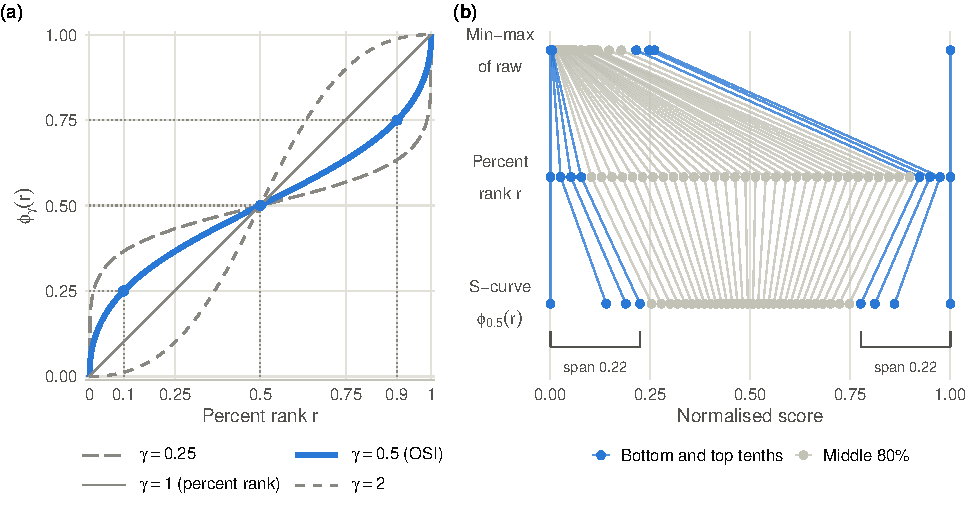
\includegraphics[width=\textwidth]{fig_scurve}
  \caption{The median-centred S-curve. Panel (a): $\Scurve(r)=r^{\gamma}/[r^{\gamma}+(1-r)^{\gamma}]$
  against the percent rank $r$ for $\gamma\in\{0.25,0.5,1,2\}$. The highlighted curve is
  $\gamma=0.5$, the value used for every component of the indices, and the marked points are
  $\Scurve(0.1)=0.25$, $\Scurve(0.5)=0.5$ and $\Scurve(0.9)=0.75$; $\gamma=1$ is the percent rank
  itself. Panel (b): 40 draws of a right-skewed variable (lognormal, log-mean 0, log-standard
  deviation 1, fixed seed) under three normalisations, with each observation joined across the
  rows: a min-max rescaling of the raw value, the percent rank $r$ of
  equation~\eqref{eq:pct_rank}, and the S-curved index of equation~\eqref{eq:scurve} computed by
  the pipeline's own function. The four lowest and four highest observations are highlighted, and
  the brackets give the span the S-curve assigns to each group. No pipeline data are used.
  Source: \texttt{scripts/paper/fig\_scurve.R}.}
  \label{fig:scurve}
\end{figure}

\paragraph{Zero anchor, comparison sets and cardinal inputs.} Ranked with positive values, tied
zeros would score mid-table (0.41 for $(0,0,0,5)$), above an economy a register omits. Measures of
activity or endowment (investment, capacity, mineral supply and export shares, reserves and
production roll-ups) therefore use an anchored form, with $m$ positive values and $\rank^{+}$ the
average-tie rank among them:
\begin{equation}\label{eq:scurve_zero}
  \Scurve^{0}[x](a)=\begin{cases}
    0, & x_a=0,\\
    \Scurve\bigl(\rank^{+}(x_a)/m\bigr), & x_a>0 .
  \end{cases}
\end{equation}
The comparison set is usually the economies observed in a pair; world-level series are ranked
across technologies, pairs or minerals and copied to every economy. Index values are positions in
a cross-section, not levels. Three $\EO$ inputs are cardinal transformations instead
(Section~\ref{sec:eo}).

% ---------------------------------------------------------------------------
\subsection{Latest-year selection}\label{subsec:norm_latest}

For every economy, technology, stage, category, variable and theme the aggregation layer keeps the
latest year present,
\begin{equation}\label{eq:latest_year}
  y^{*}_{itskvh}=\max\{y:\ \text{a row }(i,t,s,k,v,h,y)\text{ exists}\},\qquad
  x^{h}_{itskv}\equiv x^{h}_{itskv,y^{*}_{itskvh}} ,
\end{equation}
before imputation. It is a rule about the freshest information on each quantity, not a common
reference year: 60 percent of the $\ES$ cells and 92 percent of the $\EO$ cells of the eleven
headline technologies combine components from more than one year, with at most 3 distinct years in
an $\ES$ cell and 6 in an $\EO$ cell (4 once the projection horizons after 2026 of the outlook
series are set aside).

% ---------------------------------------------------------------------------
\subsection{Missing data: observed-only imputation}\label{subsec:norm_missing}

Each pair's table is completed to the product of the economies in any of the pillar's rows for
the pair and the component groups $g=(t,s,k,v,h)$ occurring there. The $\ES$ grids span 219, 215
and 219 economies at the three stages and the $\EO$ grids 219, 216 and 219. With $O_g$ the
economies observed in $g$ and $m_g$ the rule of the emitting theme (Table~\ref{tab:missing_rules}),
\begin{equation}\label{eq:impute}
  \hat x_{ig}=\begin{cases}
    x_{ig}, & i\in O_g,\\[2pt]
    0, & i\notin O_g,\ |O_g|\ge 1,\ m_g=\text{zero},\\[2pt]
    \bar x_{g}=\dfrac{1}{|O_g|}\displaystyle\sum_{j\in O_g}x_{jg},
      & i\notin O_g,\ |O_g|\ge 1,\ m_g=\text{global average},\\[8pt]
    \text{missing}, & \text{otherwise}.
  \end{cases}
\end{equation}
Imputation uses observed values only: a fill is computed from the economies observed in the group,
never from other fills, and a group observed for no economy stays missing. The zero rule, for
registers of holders, producers and investors, places an unlisted economy at the bottom, level
with an observed zero: absence from a complete register means none recorded, and leaving it
missing would reward the absence of an endowment. The global-average rule, for attributes every
economy has in some degree, places it near $1/2$, so that ``not measured'' is not read as
``worst''. Every fill is flagged and carried into the decompositions.

\begin{table}[tbp]
  \centering
  \footnotesize
  \begin{threeparttable}
    \caption{Missing-data rules by theme}\label{tab:missing_rules}
    \begin{tabularx}{\textwidth}{@{}l l c c X@{}}
      \toprule
      Theme & Category & ES & EO & Rationale \\
      \midrule
      \multicolumn{5}{@{}l}{\emph{Panel A: registers of holders, producers and investors (zero rule)}}\\
      \texttt{critical\_minerals\_production} & Production & zero & -- &
        Unlisted economy has no recorded mine output \\
      \texttt{critical\_minerals\_processing} & Foreign Dependency & zero & -- &
        Unlisted economy has no recorded supply share \\
      \texttt{critical\_minerals\_trade} & Minerals Trade & zero & -- &
        No recorded exports of the mineral \\
      \texttt{reserves} & Reserves & zero & -- &
        Reserve tables (USGS, EI, Red Book) list every holder \\
      \texttt{investment\_momentum} & Investment & zero & zero &
        Investment and capacity records; no record means none recorded \\
      \texttt{market\_share\_manufacturing} & Foreign Dependency & -- & zero &
        No recorded manufacturing share \\
      \addlinespace
      \multicolumn{5}{@{}l}{\emph{Panel B: attributes every economy has (global-average rule)}}\\
      \texttt{energy\_access\_consumption} & Energy Access & avg & avg & Coverage gap \\
      \texttt{energy\_consumption} & Energy Access, Consumption & avg & avg & Coverage gap \\
      \texttt{solar\_pv\_potential} & Reserves & avg & avg$^{a}$ &
        Every territory has some resource potential \\
      \texttt{wind\_potential} & Reserves & avg & avg$^{a}$ & As above \\
      \texttt{geothermal\_potential} & Reserves & avg & avg$^{a}$ & As above \\
      \texttt{import\_dependence} & Energy Imports & avg & -- & Coverage gap \\
      \texttt{foreign\_dependency} & Foreign Dependency & avg & -- &
        Fills economies outside the theme's roster \\
      \texttt{trade\_concentration} & Trade & avg & -- & Coverage gap \\
      \texttt{export\_feasibility} & Trade & -- & avg & Coverage gap \\
      \texttt{energy\_prices} & Energy Prices & avg & avg &
        World series; the mean is the common value \\
      \texttt{future\_demand} & Technology Demand & -- & avg & Market-level outlooks \\
      \texttt{overcapacity\_premium} & Technology Demand & -- & avg & Market-level outlooks \\
      \texttt{technological\_readiness} & Technological Readiness & -- & avg &
        Technology-level value \\
      \texttt{cost\_competitiveness} & Cost Competitiveness & -- & avg & Coverage gap \\
      \texttt{production\_depth\_momentum} & Production & -- & avg & Coverage gap \\
      \addlinespace
      \multicolumn{5}{@{}l}{\emph{Panel C: no rule (missing values stay missing)}}\\
      \texttt{lcoe\_competitiveness} & Cost Competitiveness & -- & none &
        Uncovered markets scored on the other cost components \\
      \bottomrule
    \end{tabularx}
    \begin{tablenotes}[flushleft]\footnotesize
      \item \emph{Notes:} ``zero'' assigns the bottom of the index scale and ``avg'' the mean of
      the observed index values within the technology$\times$stage$\times$category$\times$%
      variable$\times$theme group, equation~\eqref{eq:impute}; either rule applies only in groups
      where at least one economy is observed. ``--'': the theme is not an input to the pillar.
      Source: \texttt{config/missing\_data.yml}.
      \item[$a$] Inert: the potential themes supply only the Reserves category, which $\EO$ does
      not score.
    \end{tablenotes}
  \end{threeparttable}
\end{table}

% ---------------------------------------------------------------------------
\subsection{Category scores and available-case aggregation}\label{subsec:norm_pillar}

A category is scored by a configured overall variable, the unweighted mean of its components
present in the cell (a component reported by several themes is first averaged across them),
\begin{equation}\label{eq:overall}
  c_{kits}=\frac{1}{|\mathcal V^{*}_{kits}|}\sum_{v\in\mathcal V^{*}_{kits}}\tilde x_{itsv},
  \qquad
  \mathcal V^{*}_{kits}=\{v\in\mathcal V_{k}:\ \tilde x_{itsv}\text{ not missing}\},
\end{equation}
which is $c_{itsk}$ of equation~\eqref{eq:fw_category} with the category index written first. With
$K_{its}$ the categories observed in the cell and $w_k$ the nominal weights of
Table~\ref{tab:category_weights}, the pillar is the available-case weighted mean
\begin{equation}\label{eq:pillar}
  \ES_{its}=\frac{\sum_{k\in K_{its}}w_k\,c_{kits}}{\sum_{k\in K_{its}}w_k}
  =\sum_{k\in K_{its}}\omega_{kits}\,c_{kits},
\end{equation}
\begin{equation}\label{eq:effective_weight}
  \omega_{kits}=\begin{cases}
    w_k\big/\sum_{k'\in K_{its}}w_{k'}, & k\in K_{its},\\
    0, & k\notin K_{its},
  \end{cases}
\end{equation}
and identically for $\EO_{its}$. The rule is equivalent to imputing an unobserved category at the
cell's own mean; zero-filling would instead penalise coverage rather than performance. The pillar
is a weighted mean of S-curved scores, not itself a percentile.

\begin{table}[tbp]
  \centering
  \small
  \begin{threeparttable}
    \caption{Nominal category weights}\label{tab:category_weights}
    \begin{tabular}{@{}l S[table-format=2.0] S[table-format=1.3] @{\hspace{2.5em}} l S[table-format=2.0] S[table-format=1.3]@{}}
      \toprule
      \multicolumn{3}{@{}c}{Energy Security} & \multicolumn{3}{c@{}}{Economic Opportunity}\\
      \cmidrule(r){1-3}\cmidrule(l){4-6}
      {Category} & {$w_k$} & {Share} & {Category} & {$w_k$} & {Share} \\
      \midrule
      Foreign Dependency & 6 & 0.143 & Technology Demand       & 4 & 0.133 \\
      Production         & 6 & 0.143 & Trade                   & 3 & 0.100 \\
      Consumption        & 5 & 0.119 & Production              & 3 & 0.100 \\
      Energy Imports     & 4 & 0.095 & Energy Prices           & 3 & 0.100 \\
      Reserves           & 4 & 0.095 & Investment              & 3 & 0.100 \\
      Trade              & 4 & 0.095 & Energy Access           & 3 & 0.100 \\
      Minerals Trade     & 4 & 0.095 & Foreign Dependency      & 3 & 0.100 \\
      Energy Access      & 4 & 0.095 & Cost Competitiveness    & 3 & 0.100 \\
      Investment         & 3 & 0.071 & Consumption             & 3 & 0.100 \\
      Energy Prices      & 2 & 0.048 & Technological Readiness & 2 & 0.067 \\
      \midrule
      Total              & 42 & 1.000 & Total                  & 30 & 1.000 \\
      \bottomrule
    \end{tabular}
    \begin{tablenotes}[flushleft]\footnotesize
      \item \emph{Notes:} Share is $w_k/\sum_{k'}w_{k'}$, the weight a category would receive in
      a cell in which all ten are observed; no cell observes all ten. The weight applied in a cell
      is $\omega_{kits}$ of equation~\eqref{eq:effective_weight}. Source: \texttt{config/weights.yml}.
    \end{tablenotes}
  \end{threeparttable}
\end{table}

\paragraph{Composition differs across pairs, not within them.} Because every theme but the
levelised-cost theme carries a rule, all scored economies share one category set in all of the 30
$\ES$ pairs and all of the 33 $\EO$ pairs (Online Appendix~\ref{oa:normalization}): within-pair
comparisons are comparisons of one construct. Across pairs a cell has between 1 and 7 observed
categories in $\ES$ (median 3; 21 percent of cells have a single category) and between 2 and 7 in
$\EO$ (median 6). The effective weights therefore depart far from the nominal ones
(Figure~\ref{fig:method_weights}): $\ES$ Trade, nominally 0.095, carries 0.59 at the midstream
stage and Consumption (0.119) 0.49 downstream, the gap between nominal and effective importance
that \citet{paruolo2013ratings} stress. A category constant within a pair, such as Energy Prices or
Technological Readiness, makes the pillar an affine function of the pillar without it,
\begin{equation}\label{eq:affine_constant}
  \ES_{its}=\omega_{kts}\,\bar c_{kts}+(1-\omega_{kts})\,\ES^{(-k)}_{its},
\end{equation}
which shifts levels without reordering economies and matters only where levels are compared
across pairs, as in the Strategic Index (Section~\ref{sec:strategic}). The weights are normative
\citep{decancq2013weights}; Section~\ref{sec:robustness} varies them.

\begin{figure}[tbp]
  \centering
  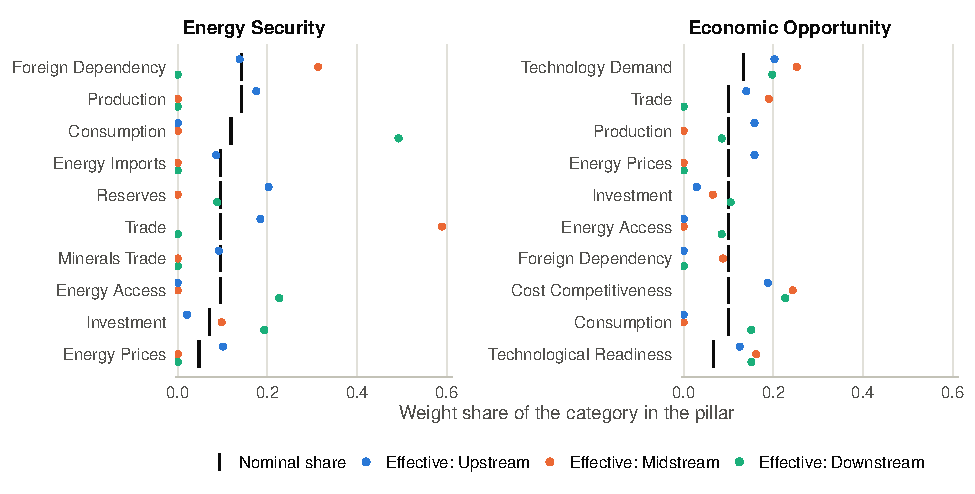
\includegraphics[width=\textwidth]{method_weights}
  \caption{Nominal and effective category weights. Black ticks: nominal share
  $w_k/\sum_{k'}w_{k'}$ over the ten categories of the pillar (\texttt{config/weights.yml};
  Table~\ref{tab:category_weights}). Dots: mean effective weight $\omega_{kits}$
  (equation~\eqref{eq:effective_weight}) over the scored cells of the eleven headline
  technologies at each stage, with $\omega_{kits}=0$ where the category is not observed. A dot
  at zero marks a category that is never observed at that stage. The effective weights of a
  stage, like the nominal shares, sum to one over the categories. A dot to the right of the
  tick means that the available-case rule gives the category more weight than its nominal share.
  Cells: 2,181, 2,002 and 2,049 for $\ES$ and 2,394, 2,346 and 2,391 for $\EO$ (upstream,
  midstream, downstream). Source: category contributions in
  \texttt{data/processed/outputs/index\_outputs.rds}; \texttt{scripts/paper/fig\_method.R}.}
  \label{fig:method_weights}
\end{figure}

% ---------------------------------------------------------------------------
\subsection{Exact decompositions}\label{subsec:norm_decomposition}

With $C_{kits}=\omega_{kits}c_{kits}$ and $\lambda_{vkits}=1/|\mathcal V^{*}_{kits}|$ for a present
component (0 otherwise), every pillar value decomposes exactly into category and variable
contributions,
\begin{equation}\label{eq:cat_decomp}
  \ES_{its}=\sum_{k\in\Cats^{P}}C_{kits},\qquad \sum_{k\in\Cats^{P}}\omega_{kits}=1 ,
\end{equation}
\begin{equation}\label{eq:var_decomp}
  \ES_{its}=\sum_{k\in\Cats^{P}}\sum_{v\in\mathcal V_{k}}
    \underbrace{\omega_{kits}\,\lambda_{vkits}\,\tilde x_{itsv}}_{\text{contribution of }v},
  \qquad
  \sum_{k}\sum_{v}\omega_{kits}\,\lambda_{vkits}=1 .
\end{equation}
The largest absolute difference between the index and the sum of its contributions is exactly
zero for the category decomposition and $1.1\times10^{-16}$ for the variable decomposition, in
both pillars (7,794 $\ES$ and 7,661 $\EO$ cells, all technologies), so the attributions of
Sections~\ref{sec:es} and~\ref{sec:eo} are exact.

% ---------------------------------------------------------------------------
\subsection{The imputed weight share}\label{subsec:norm_diagnostics}

The share of a cell's weight carried by imputed components is
\begin{equation}\label{eq:imputed_share}
  \iota_{its}=\sum_{k}\sum_{v}\omega_{kits}\,\lambda_{vkits}\,
    \1\bigl[\tilde x_{itsv}\text{ imputed}\bigr]\in[0,1],
\end{equation}
counting zero and average fills alike; a world-level series copied to every economy counts as
observed. Imputed components carry on average 31 percent of the weight of an $\ES$ cell and 43
percent of an $\EO$ cell (medians 0.26 and 0.44; Figure~\ref{fig:method_imputation}). The $\ES$
burden is heaviest upstream (0.41, against 0.23 and 0.27), where Reserves, zero-filled for
economies absent from the registers, is imputed at 0.84; the $\EO$ burden is flat across stages
(0.41, 0.44, 0.43). No $\ES$ cell and 24 $\EO$ cells (the Isle of Man 14, Puerto Rico 8,
Liechtenstein 2) rest entirely on imputation. All 30 $\ES$ and 33 $\EO$ headline pairs vary across
economies.

\begin{figure}[tbp]
  \centering
  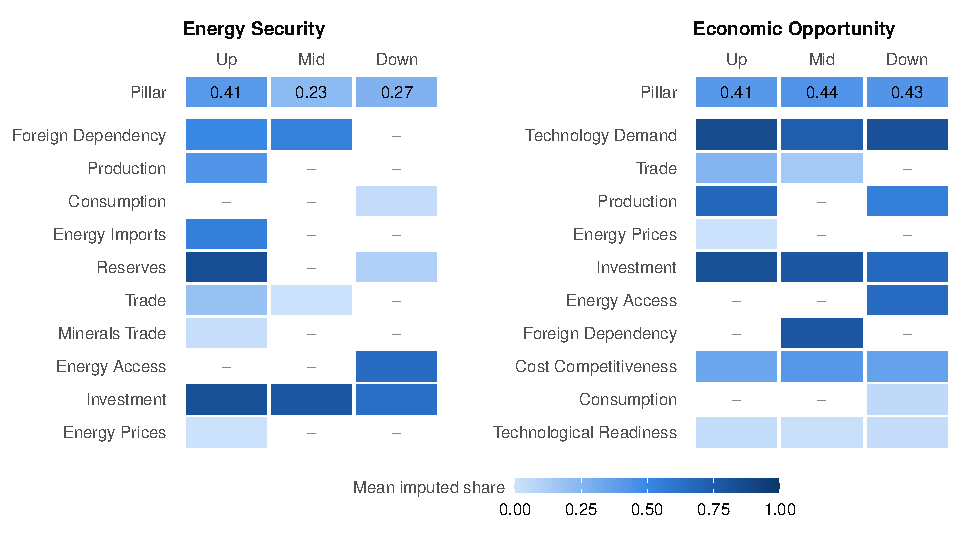
\includegraphics[width=\textwidth]{method_imputation}
  \caption{Imputation burden by category and stage. Category rows: the mean, over the headline
  cells in which the category is observed, of the share of the category score carried by
  imputed components, $\sum_v\lambda_{vkits}\1[\tilde x_{itsv}\text{ imputed}]$. Pillar row
  (with values): the mean imputed weight share $\iota_{its}$ of
  equation~\eqref{eq:imputed_share} over all scored cells of the stage, which weights the
  category rows by the effective weights. Dashes mark categories that are not observed at a
  stage. A component counts as imputed when a missing-data rule of
  Table~\ref{tab:missing_rules} supplied it, zero fills included; world-level series copied to
  every economy count as observed. Online Appendix~\ref{oa:normalization} tabulates the values.
  Source: variable contributions and pillar diagnostics in
  \texttt{data/processed/outputs/index\_outputs.rds}; \texttt{scripts/paper/fig\_method.R}.}
  \label{fig:method_imputation}
\end{figure}

% ---------------------------------------------------------------------------
\subsection{The rankability rule}\label{subsec:norm_rankability}

Every cell the sources reach is scored and enters the decompositions, but a cell enters a
cross-country ranking, a top-$N$ list or the Strategic Index only if it is rankable,
\begin{equation}\label{eq:rankable}
  R_{its}=\1\bigl[i\in\Countries^{\mathrm{sov}}\bigr]\;\1\bigl[\iota_{its}\le\tau\bigr],
  \qquad \tau=0.5 ,
\end{equation}
where $\Countries^{\mathrm{sov}}$ is the set of 195 sovereign states of the Correlates of War
state-system list \citep{cow2024state} (the 193 UN members, Kosovo and Taiwan). The threshold
reads as ``observed data carry at least half of the cell's weight''; values are never altered,
and the Partnership Strength Index applies the same rule to partners (Section~\ref{sec:bilateral}).

Of the 6,232 headline $\ES$ cells, 4,163 (67 percent) are rankable, 607 belonging to territories
and 1,462 to sovereign states over the threshold; in $\EO$, 4,301 of 7,131 (60 percent), with 718
and 2,112 excluded (Figure~\ref{fig:method_rankability}). The rule bites hardest in upstream $\ES$
(52 percent rankable, against 70 and 80), where the registers cover a minority of economies, and
in midstream and downstream $\EO$ (56 and 55 percent, against 70). Every sovereign state keeps a
rankable $\ES$ cell, but 17 keep no rankable $\EO$ cell (Liechtenstein, Monaco and fifteen small
island and low-income states). The rule is not level-neutral: since absence from a register scores
at the bottom, excluded cells lean insecure. Of the 5,854 candidate Strategic Index cells, the
3,154 kept have a mean security need $1-\ES$ of 0.58 and $\EO$ of 0.49, against 0.68 and 0.44 for
those removed. The rule states what the data can support rather than correcting the index;
Section~\ref{sec:robustness} reports other thresholds.

\begin{figure}[tbp]
  \centering
  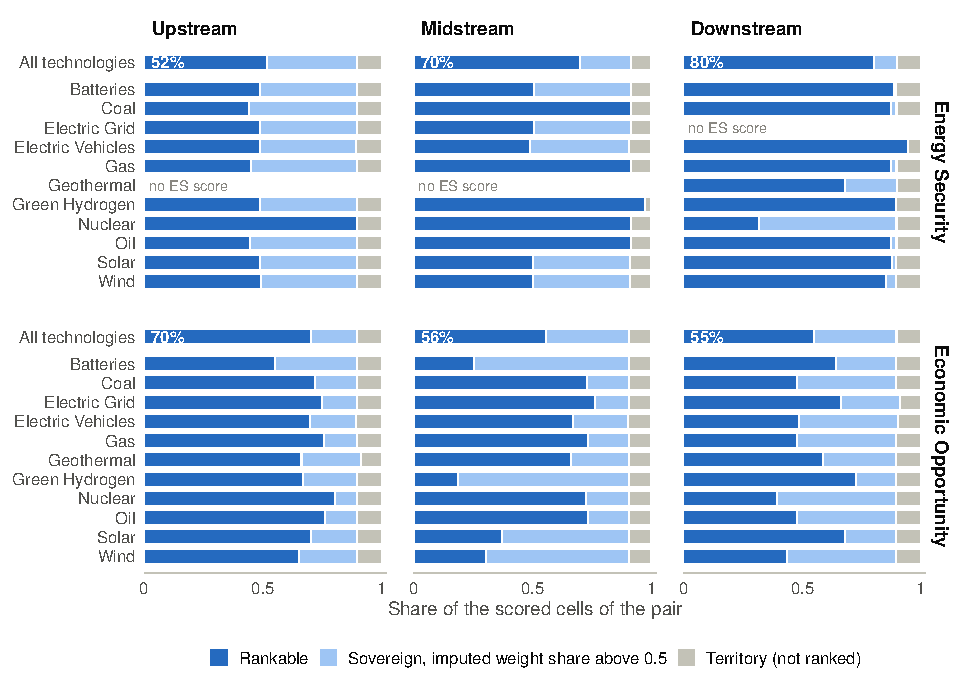
\includegraphics[width=\textwidth]{method_rankability}
  \caption{Rankability of the scored cells by technology--stage pair. Each bar divides the scored
  country--technology--stage cells of a pair into three exclusive groups: rankable cells (the
  economy is a sovereign state and the imputed weight share $\iota_{its}$ is at most
  $\tau=0.5$); cells of sovereign states with $\iota_{its}>0.5$; and cells of territories,
  special administrative regions and the West Bank and Gaza, which are scored but never ranked
  whatever their imputed share. The ``All technologies'' row pools the pairs of the stage, and its
  label gives the rankable share. Sovereignty follows the Correlates of War state-system list (195
  states: the 193 members of the United Nations, Kosovo and Taiwan). ``No ES score'' marks the
  three pairs without an $\ES$ value. Sample: the eleven headline technologies, 6,232 $\ES$ and
  7,131 $\EO$ cells; Online Appendix~\ref{oa:normalization} gives the counts by stage. Source:
  \texttt{energy\_security\_index} and \texttt{economic\_opportunity\_index} in
  \texttt{data/processed/outputs/index\_outputs.rds}; \texttt{config/rankability.yml};
  \texttt{scripts/paper/fig\_method.R}.}
  \label{fig:method_rankability}
\end{figure}

\paragraph{What the construction does not do.} The stages of a technology are scored
independently, although disruptions propagate along supply chains \citep{carvalho2021supply};
dependence across stages enters only where a variable encodes it, as the mineral-supply terms of
foreign dependency do. Section~\ref{sec:robustness} reports the test of vertical complementarities
behind this choice. Imputation assigns one value per uncovered economy, so it understates the
uncertainty of imputed cells.
